\documentclass[11pt,a4paper]{article}
\usepackage[utf8]{inputenc}
\usepackage[T1]{fontenc}
\usepackage[spanish]{babel}
\spanishplainpercent
\usepackage[a4paper,top=4cm,bottom=2.5cm,left=2.5cm,right=2.5cm,headheight=3cm,headsep=.8cm]{geometry}
\usepackage{graphicx,amsmath,amssymb,booktabs,array,siunitx,multirow,float,caption,subcaption}
\usepackage[table]{xcolor}
\usepackage{fancyhdr,lastpage,enumitem,listings,microtype}
\microtypesetup{expansion=false}
\usepackage[colorlinks=true,linkcolor=blue!50!black,urlcolor=blue!50!black,citecolor=blue!50!black]{hyperref}
\graphicspath{{./imagenes/}}
\sisetup{output-decimal-marker={,},group-separator={.}}
\captionsetup{font=small,labelfont=bf}
\makeatletter
\newcommand{\inputtablerows}[1]{\@@input #1 }
\makeatother

\lstdefinestyle{python}{language=Python,basicstyle=\ttfamily\footnotesize,
 keywordstyle=\color{blue!70!black}\bfseries,commentstyle=\color{gray!70!black}\itshape,
 stringstyle=\color{red!60!black},showstringspaces=false,numbers=left,
 numberstyle=\tiny\color{gray},frame=single,rulecolor=\color{gray!40},breaklines=true,tabsize=4,
 literate={á}{{\'a}}1 {é}{{\'e}}1 {í}{{\'i}}1 {ó}{{\'o}}1 {ú}{{\'u}}1 {ñ}{{\~n}}1}
\lstset{style=python}

% Datos del informe (plantilla)
\newcommand{\TituloInforme}{Práctica No. 4:}
\newcommand{\NombrePractica}{Simulación de eventos discretos}
\newcommand{\NombreUniversidad}{Universidad de los Llanos}
\newcommand{\NombreFacultad}{Facultad de Ciencias Básicas e Ingenierías}
\newcommand{\NombrePrograma}{Programa de Ingeniería de Sistemas}
\newcommand{\NombreCurso}{Simulación Computacional}
\newcommand{\TipoDocumento}{Informe de Laboratorio}
\newcommand{\FechaInforme}{Septiembre de 2026}
\newcommand{\Vacio}{}
\newcommand{\AlumnoUno}{J. Gregorio Delgado}
\newcommand{\CodUno}{160005010}
\newcommand{\AlumnoDos}{} \newcommand{\CodDos}{}
\newcommand{\AlumnoTres}{} \newcommand{\CodTres}{}
\newcommand{\AlumnoCuatro}{} \newcommand{\CodCuatro}{}

% Marcador visible para secciones pendientes (eliminar al completar)
\newcommand{\Pendiente}[1]{\par\noindent\colorbox{yellow!30}{\parbox{\dimexpr\textwidth-2\fboxsep}{\small\textbf{Pendiente:} #1}}\par}

\newcommand{\LogoUniversidad}{%
 \IfFileExists{../logo.png}
 {\includegraphics[width=3cm,height=2.7cm,keepaspectratio]{../logo.png}}
 {\colorbox{gray!15}{\parbox[c][2.4cm][c]{3cm}{\centering\footnotesize Logo institucional}}}}
\pagestyle{fancy}\fancyhf{}\renewcommand{\headrulewidth}{0pt}
\fancyhead[L]{\parbox[c][2.8cm][c]{3.2cm}{\centering\LogoUniversidad}}
\fancyhead[C]{\parbox[c][2.8cm][c]{\dimexpr(\textwidth-4cm)/2\relax}{\centering\footnotesize
 \textbf{\MakeUppercase{\NombreUniversidad}}\\[2pt]Facultad de Ciencias Básicas e Ingenierías}}
\fancyhead[R]{\parbox[c][2.8cm][c]{\dimexpr(\textwidth-4cm)/2\relax}{\raggedleft\footnotesize
 Curso: \NombreCurso\\[2pt]\textbf{\TipoDocumento}}}
\fancyfoot[C]{\small Página \thepage\ de \pageref{LastPage}}

\begin{document}
\begin{center}
 {\LARGE\bfseries \TituloInforme}\\[6pt]
 {\normalsize\itshape \NombrePractica}\\[16pt]
 {\large \AlumnoUno\textsuperscript{1}}\\[12pt]
 {\small 1. Código: \CodUno, Ingeniería de Sistemas.}\\[10pt]
 {\small \NombreFacultad. \NombrePrograma.}\\[4pt]
 {\small Fecha: \FechaInforme}
\end{center}

\vspace{.4cm}\noindent\rule{\textwidth}{.6pt}
\begin{abstract}
Se aplicó la metodología de simulación de eventos discretos a dos sistemas de espera
del capítulo 5 de Ríos et al.\ \cite{rios2008}: una línea de espera con un servidor
(G/G/1) y una red de tres colas. Ambos modelos se reimplementaron con programación de
sucesos y se corrigieron errores de contabilidad de los notebooks base. Se simularon dos
escenarios por modelo con 10 y 20 réplicas independientes, respectivamente, y se
estimaron medias, desviaciones estándar e intervalos de confianza al 95\,\%. Todos los
escenarios de la G/G/1 y el escenario A de la red tienen intensidad de tráfico mayor que
uno, y una aproximación de flujo reproduce sus medidas de congestión. En el escenario B de
la red, el servicio dependiente del estado estabiliza el tercer nodo. También se implementó
un modelo de inventario probabilístico con política de punto de pedido y se corrigieron
errores de su pseudocódigo. Con la política dada se satisface al 85,6\,\% de los clientes y
el inventario está vacío el 12,4\,\% del tiempo. Un punto de pedido cercano a la demanda
esperada durante la entrega más una desviación estándar eleva el servicio al 95\,\%. Por
último, se implementaron los tutoriales y siete ejemplos oficiales del framework SimPy, y
se construyeron desde cero Job Shop y Lead Acid Battery Production en AnyLogic, con
20 réplicas por modelo. Bank Office se conservó como trabajo previo del estudiante;
Subway Entrance e Intersection se excluyeron del alcance solicitado.

\medskip\noindent\textbf{Palabras clave ---} eventos discretos, teoría de colas, G/G/1,
red de colas, intervalos de confianza, inventario, SimPy, AnyLogic.
\end{abstract}
\rule{\textwidth}{.6pt}

\section{Objetivos}
\begin{itemize}
 \item Introducir el paradigma de simulación de eventos discretos mediante sus elementos,
 diseño, metodología de modelado e implementación.
 \item Apropiar la metodología a partir de dos casos de uso: un sistema de línea de
 espera con un servidor y una red de colas.
 \item Implementar la metodología en un caso de estudio de inventario probabilístico.
 \item Implementar casos de estudio en frameworks y software de simulación de eventos
 discretos: SimPy y AnyLogic.
\end{itemize}

\section{Consulta previa}
\begin{enumerate}[label=\arabic*.]
 \item \textbf{Paradigma de simulación de eventos discretos (SED).} El estado del sistema
 cambia solo en instantes aislados, llamados sucesos o eventos, y permanece constante entre
 ellos. Por eso el reloj no avanza en pasos fijos: salta de un suceso al siguiente
 (\emph{avance al próximo suceso}), y el costo computacional depende del número de sucesos,
 no de la duración simulada.
 \item \textbf{Elementos y metodología de modelado.} Los elementos son las
 \emph{entidades} (clientes, vehículos) con sus \emph{atributos}; las \emph{variables de
 estado} (p.\,ej.\ número en cola); los \emph{sucesos} (llegada, fin de servicio) con sus
 rutinas; el \emph{reloj}; la \emph{lista de sucesos} futuros; los \emph{contadores
 estadísticos}; y las \emph{rutinas de inicialización e informe}. La metodología sigue
 estos pasos: formular el problema, identificar entidades, estados y sucesos, construir el
 grafo de sucesos, codificar las rutinas, verificar y validar, diseñar los experimentos
 (réplicas, horizonte) y analizar las salidas estadísticamente \cite{rios2008}.
 \item \textbf{Sistema de cola simple.} Es un único servidor con una cola FIFO: los
 clientes llegan, esperan si el servidor está ocupado, son atendidos y salen. En notación
 de Kendall, G/G/1 indica tiempos entre llegadas y de servicio con distribución general y un
 servidor. Se caracteriza por la intensidad de tráfico $\rho=\lambda\,E[S]$: solo si
 $\rho<1$ existe un régimen estacionario.
 \item \textbf{Red de colas.} Es un conjunto de nodos de servicio interconectados en el que
 los clientes, al salir de un nodo, se dirigen a otro según reglas de enrutamiento (con
 frecuencia probabilísticas) o abandonan el sistema. La salida de un nodo es la llegada de
 otro, así que la congestión se propaga y el nodo con mayor utilización actúa como cuello
 de botella.
 \item \textbf{Inventario probabilístico.} Es un modelo de gestión de existencias con
 demanda y/o tiempos de reposición aleatorios. La política de pedidos (cuándo y cuánto
 pedir) se evalúa según los costos de almacenamiento, los costos de pedido, los ingresos por
 ventas y el nivel de servicio (demanda satisfecha y rupturas de inventario).
 \item \textbf{SimPy.} Es un framework de SED para Python orientado a procesos. Cada
 entidad es una función generadora que cede (\texttt{yield}) eventos al
 \texttt{Environment}: esperas (\texttt{timeout}), recursos (\texttt{Resource},
 \texttt{Container}, \texttt{Store}), otros procesos o condiciones. El entorno gestiona la
 lista de eventos y el reloj \cite{simpydocs,scherfke2014}.
 \item \textbf{AnyLogic para SED.} Es un software de simulación multimétodo. En AnyLogic,
 los modelos de eventos discretos se construyen con diagramas de flujo de la
 \emph{Process Modeling Library} (bloques \texttt{Source}, \texttt{Queue},
 \texttt{Delay}, \texttt{Service}, \texttt{Sink}, recursos) conectados sobre un
 espacio animado 2D/3D. La versión PLE es gratuita para uso educativo \cite{anylogichelp}.
\end{enumerate}

\section{Fundamento teórico}
\subsection{Programación de sucesos}
Ambos modelos de colas se implementan con el esquema de programación de sucesos de
\cite[Sec.~5.4]{rios2008}. La lista de sucesos guarda el instante del próximo suceso de
cada tipo (vale $\infty$ si no está programado). En cada iteración se toma el mínimo, se
avanza el reloj hasta él y se ejecuta la rutina correspondiente, que actualiza el estado y
programa nuevos sucesos. La simulación admite llegadas solo durante $[0,T]$ y termina cuando
la lista queda vacía. Así, todos los clientes que entraron completan su servicio y puede
medirse $T_p=\max(0,t_{fin}-T)$.

\subsection{Medidas de desempeño}
Para $N$ clientes con llegada $a_j$, salida $d_j$ y servicio $s_j$, los tiempos medios en
el sistema y en cola son
\begin{equation}
 \bar W=\frac1N\sum_{j=1}^N(d_j-a_j),\qquad \bar W_q=\frac1N\sum_{j=1}^N(d_j-a_j-s_j).
\end{equation}
El número medio de clientes en un nodo es un promedio temporal que se acumula en cada
suceso como área bajo $n(t)$:
\begin{equation}
 \bar n=\frac{1}{t_{fin}}\int_0^{t_{fin}}n(t)\,dt=\frac{1}{t_{fin}}\sum_k n(t_{k-1})\,(t_k-t_{k-1}).
 \label{eq:area}
\end{equation}

\subsection{Aproximación de flujo para sistemas saturados}
Si $\rho=\lambda/\mu>1$, la cola crece en promedio a razón de $\lambda-\mu$ clientes por
unidad de tiempo. En un horizonte $T$ se esperan unos $(\lambda-\mu)T$ clientes acumulados
en $T$, un tiempo de vaciado $T_p\approx(\lambda-\mu)T/\mu$ y una espera media en cola
$\bar W_q\approx(\lambda-\mu)T/(2\mu)$, que resulta de promediar la espera de un cliente
que llega en $t\sim U(0,T)$. Estas expresiones sirven para validar las simulaciones.

\subsection{Intervalos de confianza por réplicas independientes}
Con $R$ réplicas independientes $X_1,\dots,X_R$ de una medida, la media y la desviación
estándar muestrales son $\bar X=\frac1R\sum X_r$ y
$S=\sqrt{\frac{1}{R-1}\sum(X_r-\bar X)^2}$, y el intervalo de confianza al $95\,\%$ es
\begin{equation}
 \bar X\pm t_{0{,}975,\,R-1}\,\frac{S}{\sqrt R},\qquad t_{0{,}975,19}=2{,}093.
\end{equation}
El semiancho decrece como $1/\sqrt R$: para reducirlo a la mitad se necesitan cuatro
veces más réplicas.

\section{Equipos, materiales y herramientas}
\begin{table}[H]\centering
\caption{Recursos utilizados.}
\begin{tabular}{p{.27\textwidth}p{.6\textwidth}}\toprule
\textbf{Recurso}&\textbf{Descripción}\\\midrule
Equipo de cómputo&Computador personal.\\
Python 3.12&Implementación reproducible en el notebook \texttt{Lab4\_160005010.ipynb}.\\
Bibliotecas&NumPy, SciPy (cuantiles $t$), pandas, Matplotlib y SimPy 4.1.\\
Notebooks base&\emph{Sistema de línea de espera con un servidor -- G/G/1} y \emph{Red de Colas}.\\
AnyLogic PLE&Software de simulación para los tutoriales de la sección~5.5.\\
Fuente&Capítulo 5 de Ríos et al.\ \cite{rios2008}.\\\bottomrule
\end{tabular}\end{table}

\section{Procedimiento o metodología}
\subsection{Sistema de línea de espera con un servidor}
Se reescribió el modelo del notebook base como una función con estado local
(Listado~\ref{lst:gg1}), conservando sus dos sucesos: llegada y salida. Se detectó un error
de índices en el notebook base: las listas de llegadas, salidas y servicios se iniciaban con
un valor ficticio 0, y el promedio recorría los índices $0,\dots,N-1$. Así se incluía un
cliente inexistente con tiempo cero y se omitía el último cliente real. En la
reimplementación cada lista contiene solo clientes reales.

\begin{lstlisting}[caption={Bucle principal de la G/G/1 (programación de sucesos).},label=lst:gg1]
while t_ll < INF or t_s < INF:
    if t_ll <= t_s:                    # suceso: llegada
        t = t_ll; n += 1; llegadas.append(t)
        x = gen_llegada(rng)
        t_ll = t + x if t + x < T else INF
        if n == 1:                     # servidor libre
            y = gen_servicio(rng); servicios.append(y); t_s = t + y
    else:                              # suceso: salida
        t = t_s; n -= 1; salidas.append(t)
        if n > 0:
            y = gen_servicio(rng); servicios.append(y); t_s = t + y
        else:
            t_s = INF
\end{lstlisting}

El notebook base genera exponenciales con $X=-\ln(1-U)/\lambda$, es decir, trata $\lambda$
como tasa, y se conservó esa convención. Los escenarios fueron:
\begin{itemize}
 \item \textbf{A:} $T=40$; entre llegadas $\text{Exp}(\lambda=5)$ (media 0,2); servicio
 $\text{Exp}(\lambda=3)$ (media 0,333); $\rho=5/3\approx1{,}67$.
 \item \textbf{B:} $T=40$; entre llegadas $\text{Exp}(\lambda=1)$; servicio
 $\max(0,N(2,1))$, con media $\approx2{,}008$; $\rho\approx2{,}01$.
\end{itemize}
Se hizo una corrida detallada por escenario y luego 10 réplicas independientes. La réplica
$i$ del escenario $k$ usa la semilla $160005010+1000k+i$ con el generador PCG64 de NumPy.

\subsection{Red de colas}
El modelo del centro de diagnóstico automotriz \cite[Sec.~5.5.2]{rios2008} tiene tres nodos
FIFO de un servidor. Tras el nodo 1, cada vehículo va al nodo 2 con probabilidad 0,4 (y
luego al 3) o directamente al nodo 3 con probabilidad 0,6. El servicio del nodo 3 es
$N(\mu_{31},\sigma_{31})$ si $n_3<5$ y $N(\mu_{32},\sigma_{32})$ si $n_3\ge5$, evaluado al
iniciar cada servicio. Las normales negativas se truncan a cero. El notebook base usa
\texttt{np.random.exponential(L)}, cuyo argumento es la \emph{media}, y se conservó esa
convención (Tabla~\ref{tab:param_red}).

\begin{table}[H]\centering
\caption{Parámetros de la red de colas ($T=300$).}\label{tab:param_red}
\begin{tabular}{lcc}\toprule
\textbf{Parámetro}&\textbf{Escenario A}&\textbf{Escenario B}\\\midrule
Media entre llegadas (Exp)&2&3\\
Nodo 1: $N(\mu_1,\sigma_1)$&(2,1; 0,5)&(3,0; 1,0)\\
Nodo 2: Exp con media $\mu_2$&2,4&1,5\\
Nodo 3 si $n_3<5$: $N(\mu_{31},\sigma_{31})$&(4,1; 2,5)&(4,0; 2,0)\\
Nodo 3 si $n_3\ge5$: $N(\mu_{32},\sigma_{32})$&(3,0; 2,0)&(2,0; 1,5)\\\bottomrule
\end{tabular}\end{table}

Respecto al notebook base se hicieron tres correcciones:
\begin{enumerate}[label=(\alph*)]
 \item \textbf{Áreas de la Ecuación~\eqref{eq:area}.} El área de cada nodo solo se
 actualizaba en los sucesos que lo modificaban, pero con un intervalo medido desde el último
 suceso de \emph{cualquier} nodo. Así se perdía área y se subestimaban $\bar n_2$ y
 $\bar n_3$. Ahora, en cada suceso, se acumula el área de los tres nodos antes de cambiar el
 estado.
 \item \textbf{Tiempo en el sistema.} Se aproximaba como $\bar W_1+0{,}4\,\bar W_2+\bar W_3$.
 Ahora cada vehículo lleva un identificador y se mide exactamente su tiempo de salida menos
 su tiempo de llegada.
 \item \textbf{Registro de trayectorias.} El bucle original podía ejecutar varios sucesos
 en una iteración y registrar solo el último estado. Ahora se registra el estado después de
 cada suceso.
\end{enumerate}
Se hicieron 20 réplicas por escenario, con semillas $160005010+5000+1000k+i$.

\subsection{Inventario probabilístico}
Se implementó el modelo de \cite[Sec.~5.6]{rios2008}. Un almacén vende un producto a $r$
por unidad. Los clientes llegan según un proceso de Poisson de tasa $\lambda$ y cada uno
demanda una cantidad aleatoria con distribución $G$. Si la demanda supera las existencias,
se vende lo que queda y se pierde el resto. La política de pedidos es periódica: cuando el
nivel $x$ es menor que $p$ y no hay pedido pendiente, se piden $P-x$ unidades, que llegan
tras un tiempo $L$ y se pagan a su llegada con costo $c(y)$. El almacenamiento cuesta una
cantidad fija por unidad y unidad de tiempo. La Tabla~\ref{tab:elem_inv} resume los
elementos del modelo.

\begin{table}[H]\centering\small
\caption{Elementos del modelo de inventario.}\label{tab:elem_inv}
\begin{tabular}{p{.22\textwidth}p{.68\textwidth}}\toprule
\textbf{Elemento}&\textbf{Descripción}\\\midrule
Variables de estado&$x$: unidades en inventario; $y$: unidades en el pedido pendiente
($y=0$ si no hay).\\
Sucesos&Llegada de cliente ($t_C$) y llegada de pedido ($t_P$).\\
Contadores&$C$ costo de pedidos, $H$ costo de almacenamiento, $R$ ingresos,
$N_{C+}$/$N_{C-}$ clientes satisfechos/no satisfechos, $t_0$ tiempo en cero.\\
Salidas&Beneficio $R-C-H$; $\%$ satisfechos $N_{C+}/(N_{C+}+N_{C-})$; $\%$ en cero
$t_0/t$.\\\bottomrule
\end{tabular}\end{table}

\paragraph{Rutinas de sucesos.} En una \emph{llegada de cliente} se hacen, en orden, estos
pasos:
\begin{enumerate}[label=\arabic*.]
 \item Se acumula el costo de almacenamiento $H\mathrel{+}=a\,x\,(t_{suc}-t)$.
 \item Se genera la demanda $D\sim G$ y se vende $\min(D,x)$.
 \item Se actualiza $N_{C+}$ o $N_{C-}$ según si la demanda se satisfizo por completo.
 \item Si $x<p$ y $y=0$, se programa un pedido de $P-x$ unidades para $t+L$.
 \item Se programa la próxima llegada si ocurre antes de $T$.
\end{enumerate}
En una \emph{llegada de pedido} se acumula $H$, se suma $c(y)$ a $C$, se hace $x\mathrel{+}=y$,
$y=0$ y, si el inventario estaba en cero, se suma a $t_0$ la duración de ese periodo.

\paragraph{Parámetros.} Los de la guía son $P_0=20$, $P=100$, $p=20$, $L=5$, $h=100$ y
$r=150$. La guía define $h$ como el \emph{valor a pagar por una unidad del producto}, por lo
que $c(y)=h\,y$ y el margen por unidad vendida es $r-h=50$. Como la guía no fija el resto,
se eligieron $T=100$ días, $\lambda=2$ clientes/día, $G$ uniforme discreta en
$\{1,\dots,5\}$ (media 3 y $E[D^2]=11$) y un costo de almacenamiento $a=1$ por unidad y
día. Con estos valores, la demanda durante el tiempo de entrega tiene media
$\mu_L=\lambda L\,E[D]=30$ y desviación $\sigma_L=\sqrt{\lambda L\,E[D^2]}\approx10{,}5$.
Como $\mu_L$ supera el punto de pedido $p=20$, cabe esperar rupturas y el porcentaje de
tiempo en cero es informativo. Se hizo una corrida detallada, 20 réplicas y dos análisis de
sensibilidad, uno sobre $\lambda$ y otro sobre $p$.

\paragraph{Correcciones al pseudocódigo del libro.}
\begin{enumerate}[label=(\alph*)]
 \item La condición de venta completa se implementó como $D\le x$, que es lo que describe
 el texto. El pseudocódigo usa $D<x$.
 \item En la venta completa se incrementa $N_{C+}$; el pseudocódigo tiene la errata
 $N_{C-}=N_{C+}+1$.
 \item El inicio de un periodo en cero se registra cuando $x$ \emph{pasa} a 0, tanto por
 venta completa como parcial. El pseudocódigo lo reinicia con cada cliente insatisfecho,
 aunque el inventario ya estuviera vacío, y lo omite cuando una venta completa agota el
 inventario. Ambos casos subestiman $t_0$.
\end{enumerate}

\subsection{Simulación de eventos discretos en SimPy}
Se instaló SimPy 4.1.2 con \texttt{pip install simpy}. Se siguieron el tutorial
\emph{SimPy in 10 minutes}, la presentación de Scherfke \cite{scherfke2014} y el notebook
\emph{Discrete-event simulation with SimPy}. Con ellos se reprodujeron funciones generadoras,
procesos con \texttt{timeout}, interacción e interrupción de procesos, recursos compartidos,
eventos de condición y el caso del buffet de la conferencia. Después se implementaron los
siete ejemplos oficiales de la documentación \cite{simpydocs}: Bank Renege, Carwash, Machine
Shop, Movie Renege, Gas Station Refueling, Process Communication y Event Latency. Se
conservaron su lógica y su semilla (\texttt{RANDOM\_SEED = 42}) y se tradujeron los mensajes
al español.

\subsection{Simulación de eventos discretos en AnyLogic}
Se usó AnyLogic PLE 8.9.10 y su ayuda oficial instalada. Se construyeron clases,
conexiones y parámetros propios desde un proyecto vacío, siguiendo las cinco fases de
Job Shop y las ocho de Lead Acid Battery Production. Los recursos 3D proceden de la
paleta estándar; la disposición espacial se adaptó para evitar superposiciones y
asegurar el alcance de las grúas. Las referencias resueltas se conservaron separadas,
sin importarlas como base de los modelos finales. Bank Office se mantuvo como trabajo
previo; Subway Entrance e Intersection quedaron fuera del alcance solicitado.

Job Shop utiliza cinco montacargas a 1 m/s, camiones cada hora con 60 pallets, tiempo
en almacén triangular de 15, 20 y 30 minutos, y dos CNC de un minuto de procesamiento.
En baterías, dos líneas preparan ánodos y cátodos en lotes de 100; un operador ensambla
15 placas de cada tipo en cinco minutos. Las cajas llegan a 10/h. Grúas y un AGV
realizan las transferencias; QA dura entre 20 y 30 segundos y rechaza el 1\,\%.
Cada línea recibe rollos de 0,075 m$^3$ cada dos horas. El curado de dos minutos es la
simplificación didáctica de la guía, distinta del curado industrial de 12--24 horas.

El experimento nativo \texttt{Estadistica} ejecutó 20 réplicas con semillas
160005011--160005030 y estado inicial vacío. Job Shop usa un horizonte de ocho horas;
baterías usa cuatro horas por el límite de cinco horas de Material Handling en PLE.
AnyLogic exportó los CSV; Python comprobó balances y calculó los IC de medias entre
réplicas con $\bar{x}\pm t_{0,975;19}s/\sqrt{20}$.

\section{Resultados y análisis}
\subsection{Sistema de línea de espera con un servidor}
La Figura~\ref{fig:gg1} muestra una corrida de cada escenario. En la corrida de A pasaron
192 clientes, el máximo en el sistema fue 70 y el último cliente salió 22,70 unidades
después de $T$, con tiempos medios de 12,45 en el sistema y 12,12 en cola. En la corrida de
B pasaron 28 clientes, con un máximo de 10, $T_p=14{,}45$ y tiempos medios de 11,05 y 9,21.
En ambos casos $n(t)$ crece hasta $T$ y luego decae linealmente, como corresponde a
$\rho>1$.

\begin{figure}[H]\centering
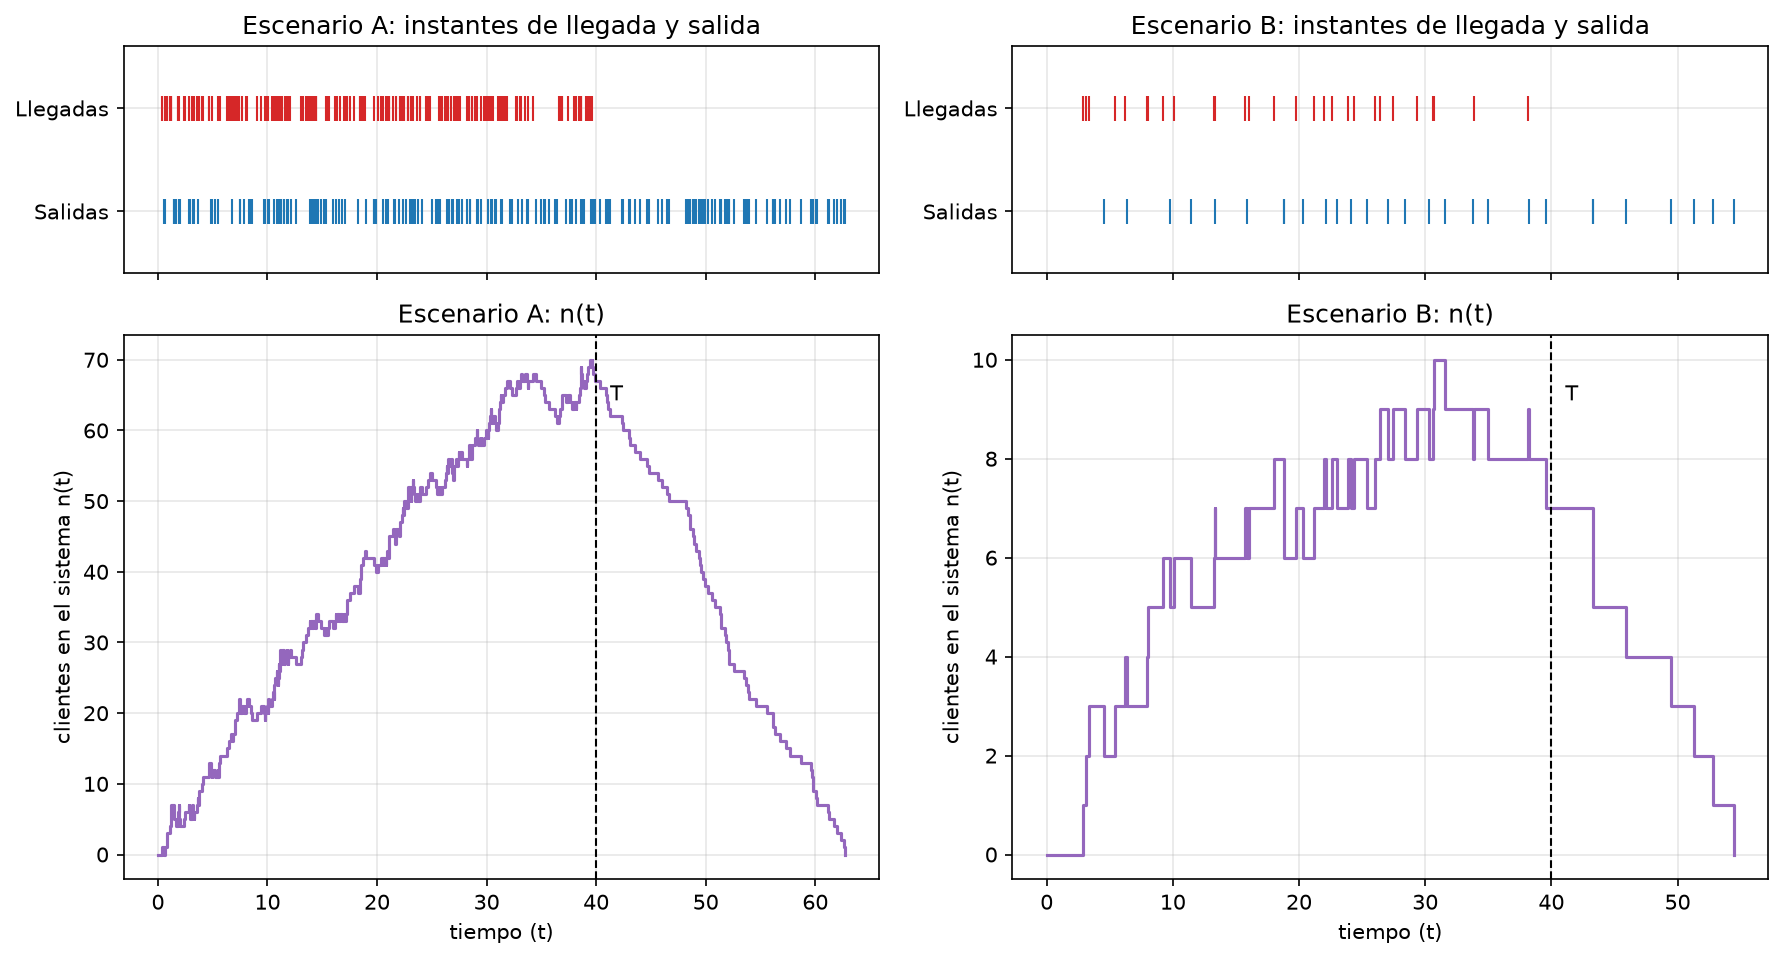
\includegraphics[width=\textwidth]{gg1_trayectorias.png}
\caption{G/G/1: instantes de llegada y salida (arriba) y número de clientes en el sistema
(abajo) para una corrida de cada escenario. La línea discontinua marca $T=40$.}\label{fig:gg1}
\end{figure}

\begin{table}[H]\centering
\caption{Medidas de desempeño para los escenarios A y B luego de 10 simulaciones
(promedio $\pm$ desviación estándar).}\label{tab:gg1}
\begin{tabular}{p{.5\textwidth}cc}\toprule
\textbf{Medida de desempeño}&\textbf{Escenario A}&\textbf{Escenario B}\\\midrule
\inputtablerows{tablas/tabla_gg1.tex}
\bottomrule
\end{tabular}\end{table}

\begin{table}[H]\centering
\caption{Validación con la aproximación de flujo (teórico / simulado); en B,
$\mu=1/2{,}008$.}\label{tab:flujo}
\begin{tabular}{lcc}\toprule
\textbf{Medida}&\textbf{Escenario A}&\textbf{Escenario B}\\\midrule
Acumulado en $T$ vs.\ $n_{max}$, $(\lambda-\mu)T$&80 / 84,5&20,1 / 20,4\\
Vaciado $T_p$, $(\lambda-\mu)T/\mu$&26,7 / 28,7&40,3 / 40,1\\
Total de clientes, $\lambda T$&200 / 200,5&40 / 38,5\\
Espera en cola, $(\lambda-\mu)T/(2\mu)$&13,3 / 14,6&20,2 / 19,7\\\bottomrule
\end{tabular}\end{table}

\paragraph{Análisis comparativo.} Ambos escenarios están saturados durante $[0,T]$, y la
aproximación de flujo (Tabla~\ref{tab:flujo}) reproduce los promedios simulados, lo que
valida la implementación. El escenario A recibe cinco veces más clientes y su cola máxima es
unas cuatro veces mayor (84,5 frente a 20,4). Aun así, cada cliente permanece menos tiempo
(15,0 frente a 21,7), porque el servicio es seis veces más rápido. El escenario B tiene
mayor intensidad de tráfico ($\rho\approx2$): su cola crece más despacio en número de
clientes, pero cada uno espera más, y el sistema tarda más en vaciarse después de $T$
(40,1 frente a 28,7). La diferencia entre tiempo en el sistema y en cola coincide con el
servicio medio: $0{,}34\approx1/3$ en A y $2{,}04\approx2{,}008$ en B. La variabilidad
relativa es mayor en B (coeficiente de variación de $T_p$ de 0,38 frente a 0,27), porque con
menos clientes cada réplica depende de pocas realizaciones. Por último, al ser $\rho>1$ no
existe estado estacionario: estas medidas dependen de $T$ y crecerían aproximadamente en
proporción si se ampliara el horizonte.

\subsection{Red de colas}
La Figura~\ref{fig:red} muestra una corrida por escenario. En A, $n_1(t)$ crece hasta
$T$ y el nodo 3 sigue acumulando vehículos incluso después de $T$, mientras se vacía el
nodo 1. El sistema tarda unas 304 unidades adicionales en vaciarse. En B, $n_1$ fluctúa sin
tendencia y $n_3$ oscila alrededor de 4--6. Las Tablas~\ref{tab:redA} y~\ref{tab:redB}
resumen las 20 réplicas, y la Figura~\ref{fig:ic} compara los intervalos.

\begin{figure}[H]\centering
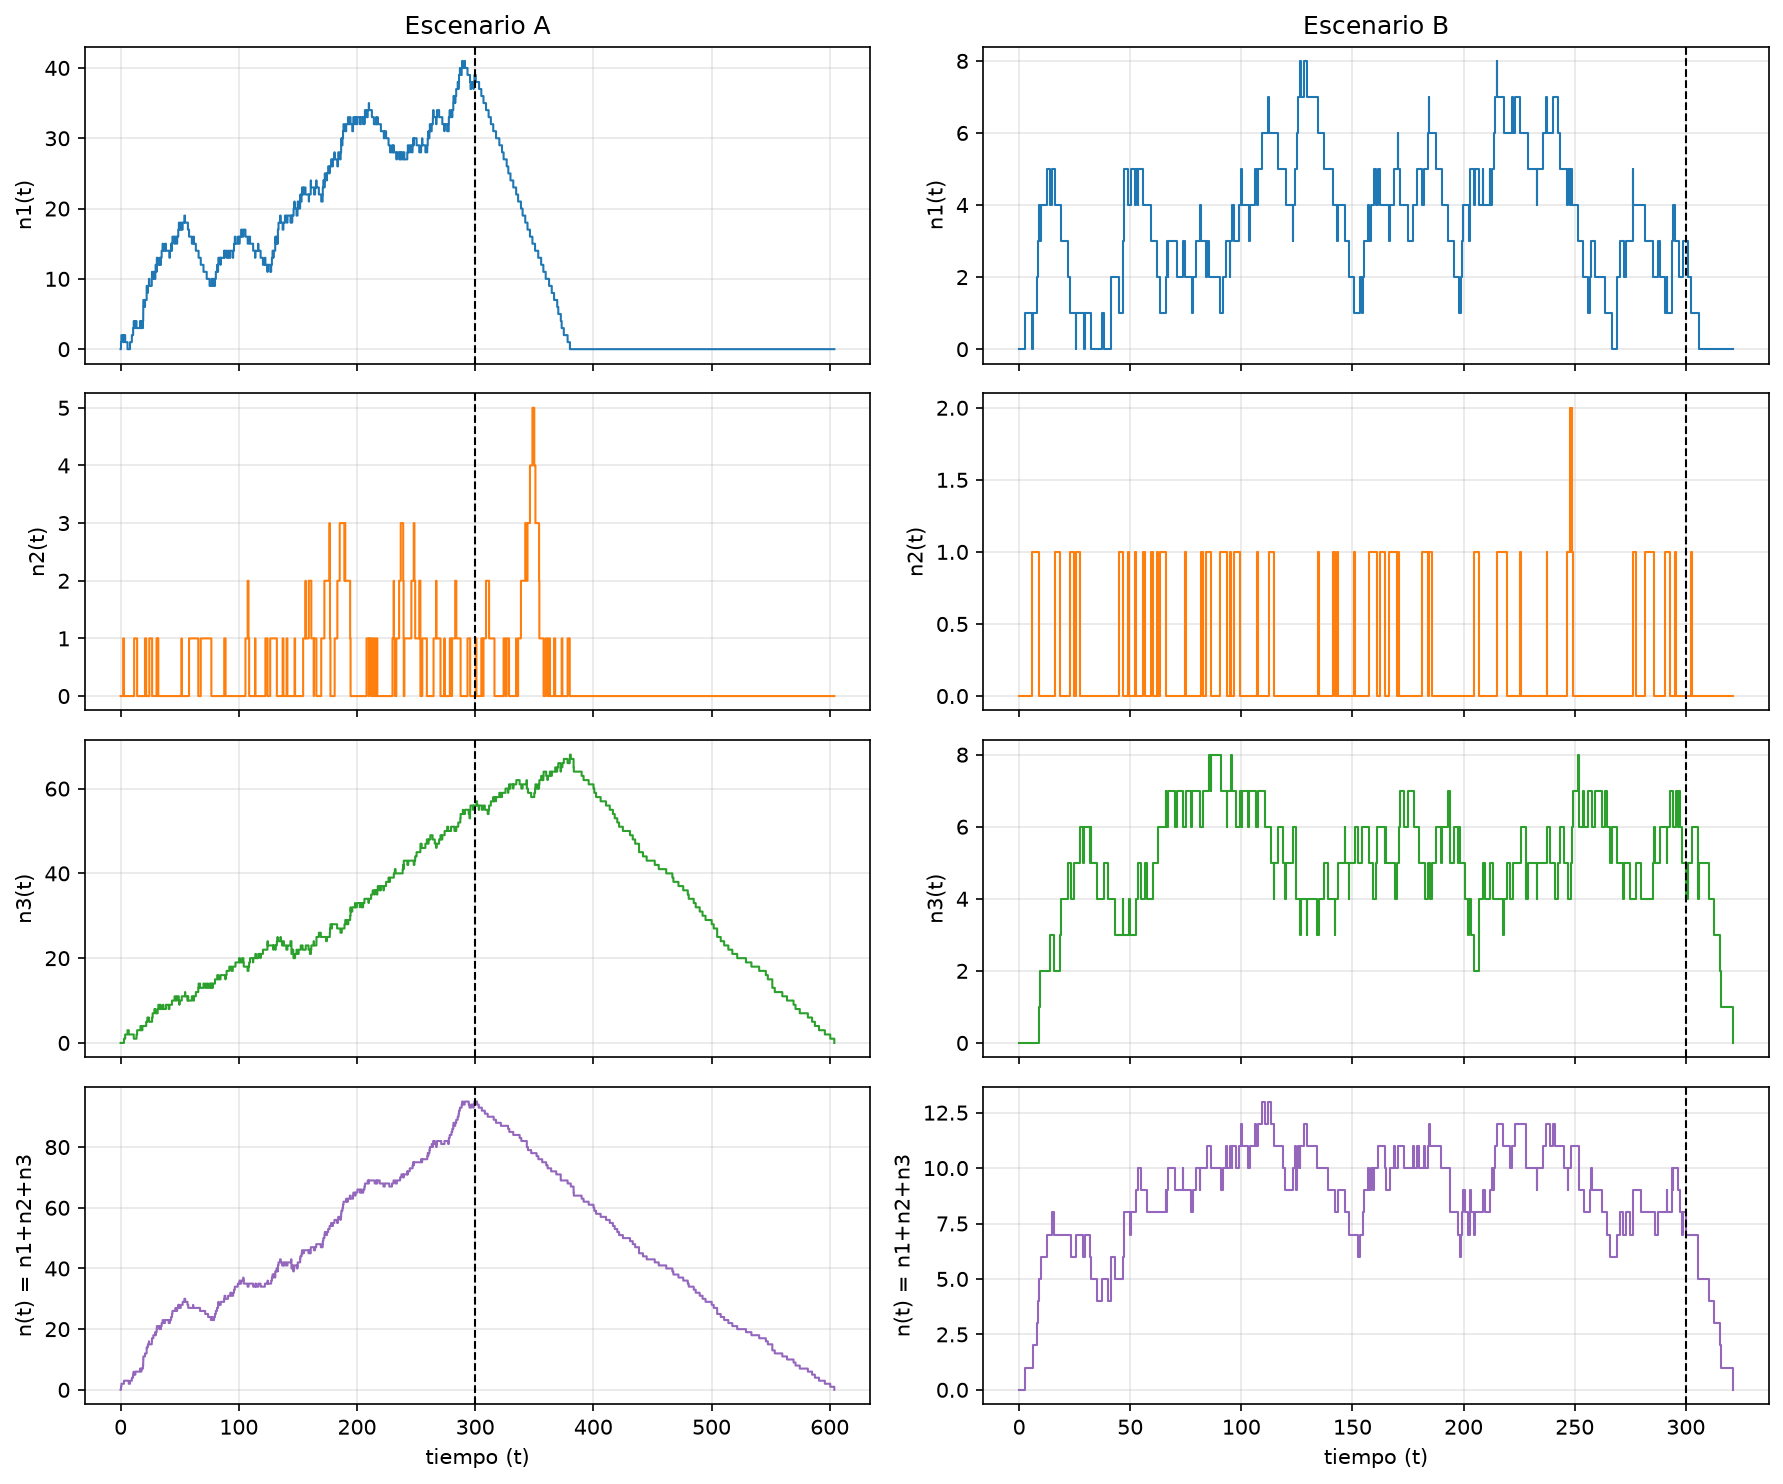
\includegraphics[width=\textwidth]{red_trayectorias.png}
\caption{Red de colas: número de vehículos en cada nodo y en el sistema para una corrida
de cada escenario. La línea discontinua marca $T=300$.}\label{fig:red}
\end{figure}

\begin{table}[H]\centering\small
\caption{Red de colas, escenario A: resultados de 20 réplicas.}\label{tab:redA}
\begin{tabular}{p{.47\textwidth}rrc}\toprule
\textbf{Medida}&\textbf{Media}&\textbf{Desv. est.}&\textbf{IC 95\,\%}\\\midrule
\inputtablerows{tablas/tabla_red_A.tex}
\bottomrule
\end{tabular}\end{table}

\begin{table}[H]\centering\small
\caption{Red de colas, escenario B: resultados de 20 réplicas.}\label{tab:redB}
\begin{tabular}{p{.47\textwidth}rrc}\toprule
\textbf{Medida}&\textbf{Media}&\textbf{Desv. est.}&\textbf{IC 95\,\%}\\\midrule
\inputtablerows{tablas/tabla_red_B.tex}
\bottomrule
\end{tabular}\end{table}

\begin{figure}[H]\centering
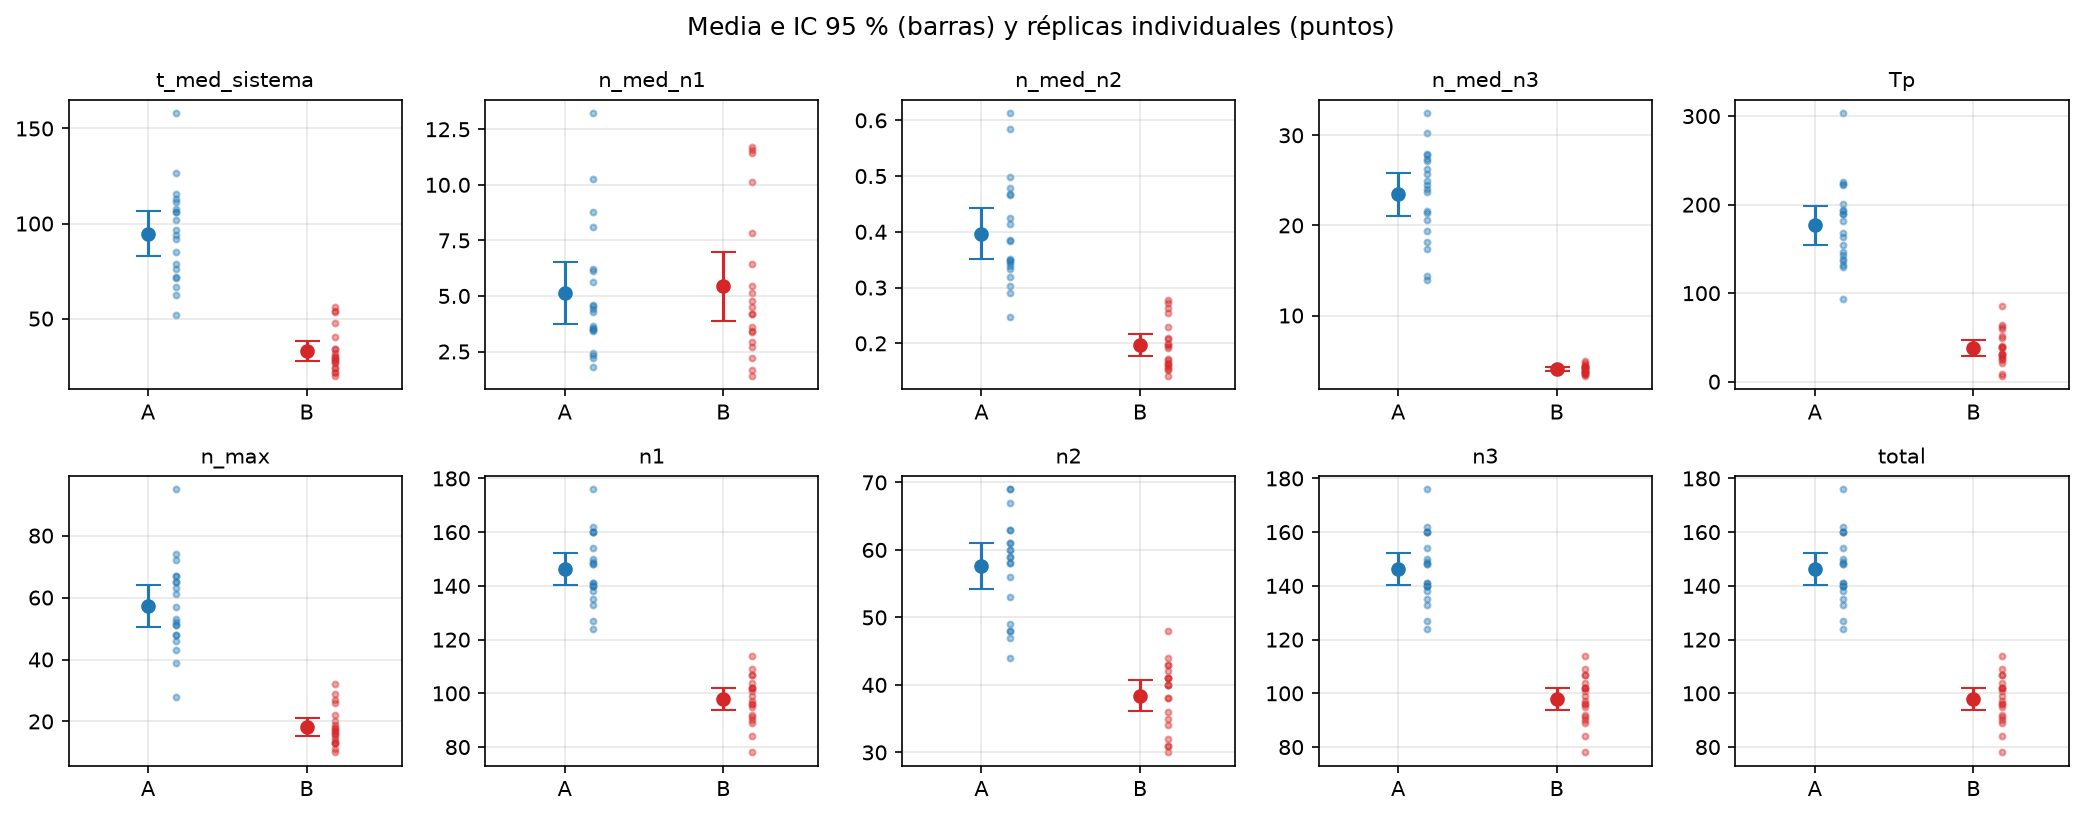
\includegraphics[width=\textwidth]{red_intervalos.png}
\caption{Media e intervalo de confianza al 95\,\% (barras) y valores de cada réplica
(puntos) por medida y escenario.}\label{fig:ic}
\end{figure}

\paragraph{Media y desviación estándar muestral.} Las utilizaciones explican los
resultados. En A, $\rho_1=1{,}05$ y el nodo 3 recibe unos $0{,}476$ vehículos por unidad
de tiempo, con utilización de 1,95 si $n_3<5$ y de 1,43 si $n_3\ge5$. Así, el nodo 3 es el
cuello de botella: acumula en promedio 23,4 vehículos y eleva el tiempo medio en el sistema
a 94,6 y el tiempo de vaciado a 176,6, ambos con gran dispersión ($S=25{,}1$ y $46{,}7$).
En B, el nodo 3 es lento con pocos vehículos ($\rho=1{,}33$) y rápido con cinco o más
($\rho=0{,}67$). Este servicio dependiente del estado mantiene $n_3$ cerca de 4--5, y
$\bar n_3=4{,}03$ con $S=0{,}44$ es la medida más estable del estudio. El nodo 1 de B, en
cambio, está en carga crítica ($\rho_1\approx1$) y es el más variable: sus réplicas van de
1,4 a 11,7. El nodo 2 está poco cargado en ambos escenarios. En B, $\bar n_2=0{,}20$
coincide con $\rho_2=0{,}2$. Los conteos confirman la lógica del modelo: $n_1=n_3=$ total en
todas las réplicas, y $n_2/n_1$ vale 0,394 (A) y 0,393 (B), frente a la probabilidad de
enrutamiento 0,4.

\paragraph{Intervalos de confianza.} Los conteos tienen intervalos estrechos (semiancho
cercano al 4\,\% de la media) que contienen el valor teórico $\lambda T$: 150 en A y 100 en
B. Las medidas de congestión tienen semianchos relativos entre 10\,\% y 29\,\%, y los
mayores corresponden a los nodos en carga crítica o inestable ($\bar n_1$ y $T_p$ en B).
Para reducirlos a la mitad harían falta unas 80 réplicas. Salvo $\bar n_1$, los intervalos
de A y B no se solapan, así que con 95\,\% de confianza A es significativamente más
congestionado. Para $\bar n_1$ los intervalos ([3,75; 6,52] y [3,87; 7,00]) se solapan casi
por completo, coherente con $\rho_1\approx1$ en ambos escenarios. Como los sistemas
saturados no tienen régimen estacionario, estos intervalos estiman el desempeño medio en el
horizonte $T=300$ partiendo de un sistema vacío, no un valor de largo plazo.

\subsection{Inventario probabilístico}
La Figura~\ref{fig:inv} reproduce, para la corrida base, la evolución de la Figura~5.9 del
libro. En esa corrida llegaron 193 clientes. Los ingresos fueron $R=77\,250$, el costo de
pedidos $C=57\,600$ y el de almacenamiento $H=3\,433$, con un beneficio de 16\,217. Se
satisfizo al 89,64\,\% de los clientes y el inventario estuvo en cero el 13,30\,\% del
tiempo.

\begin{figure}[H]\centering
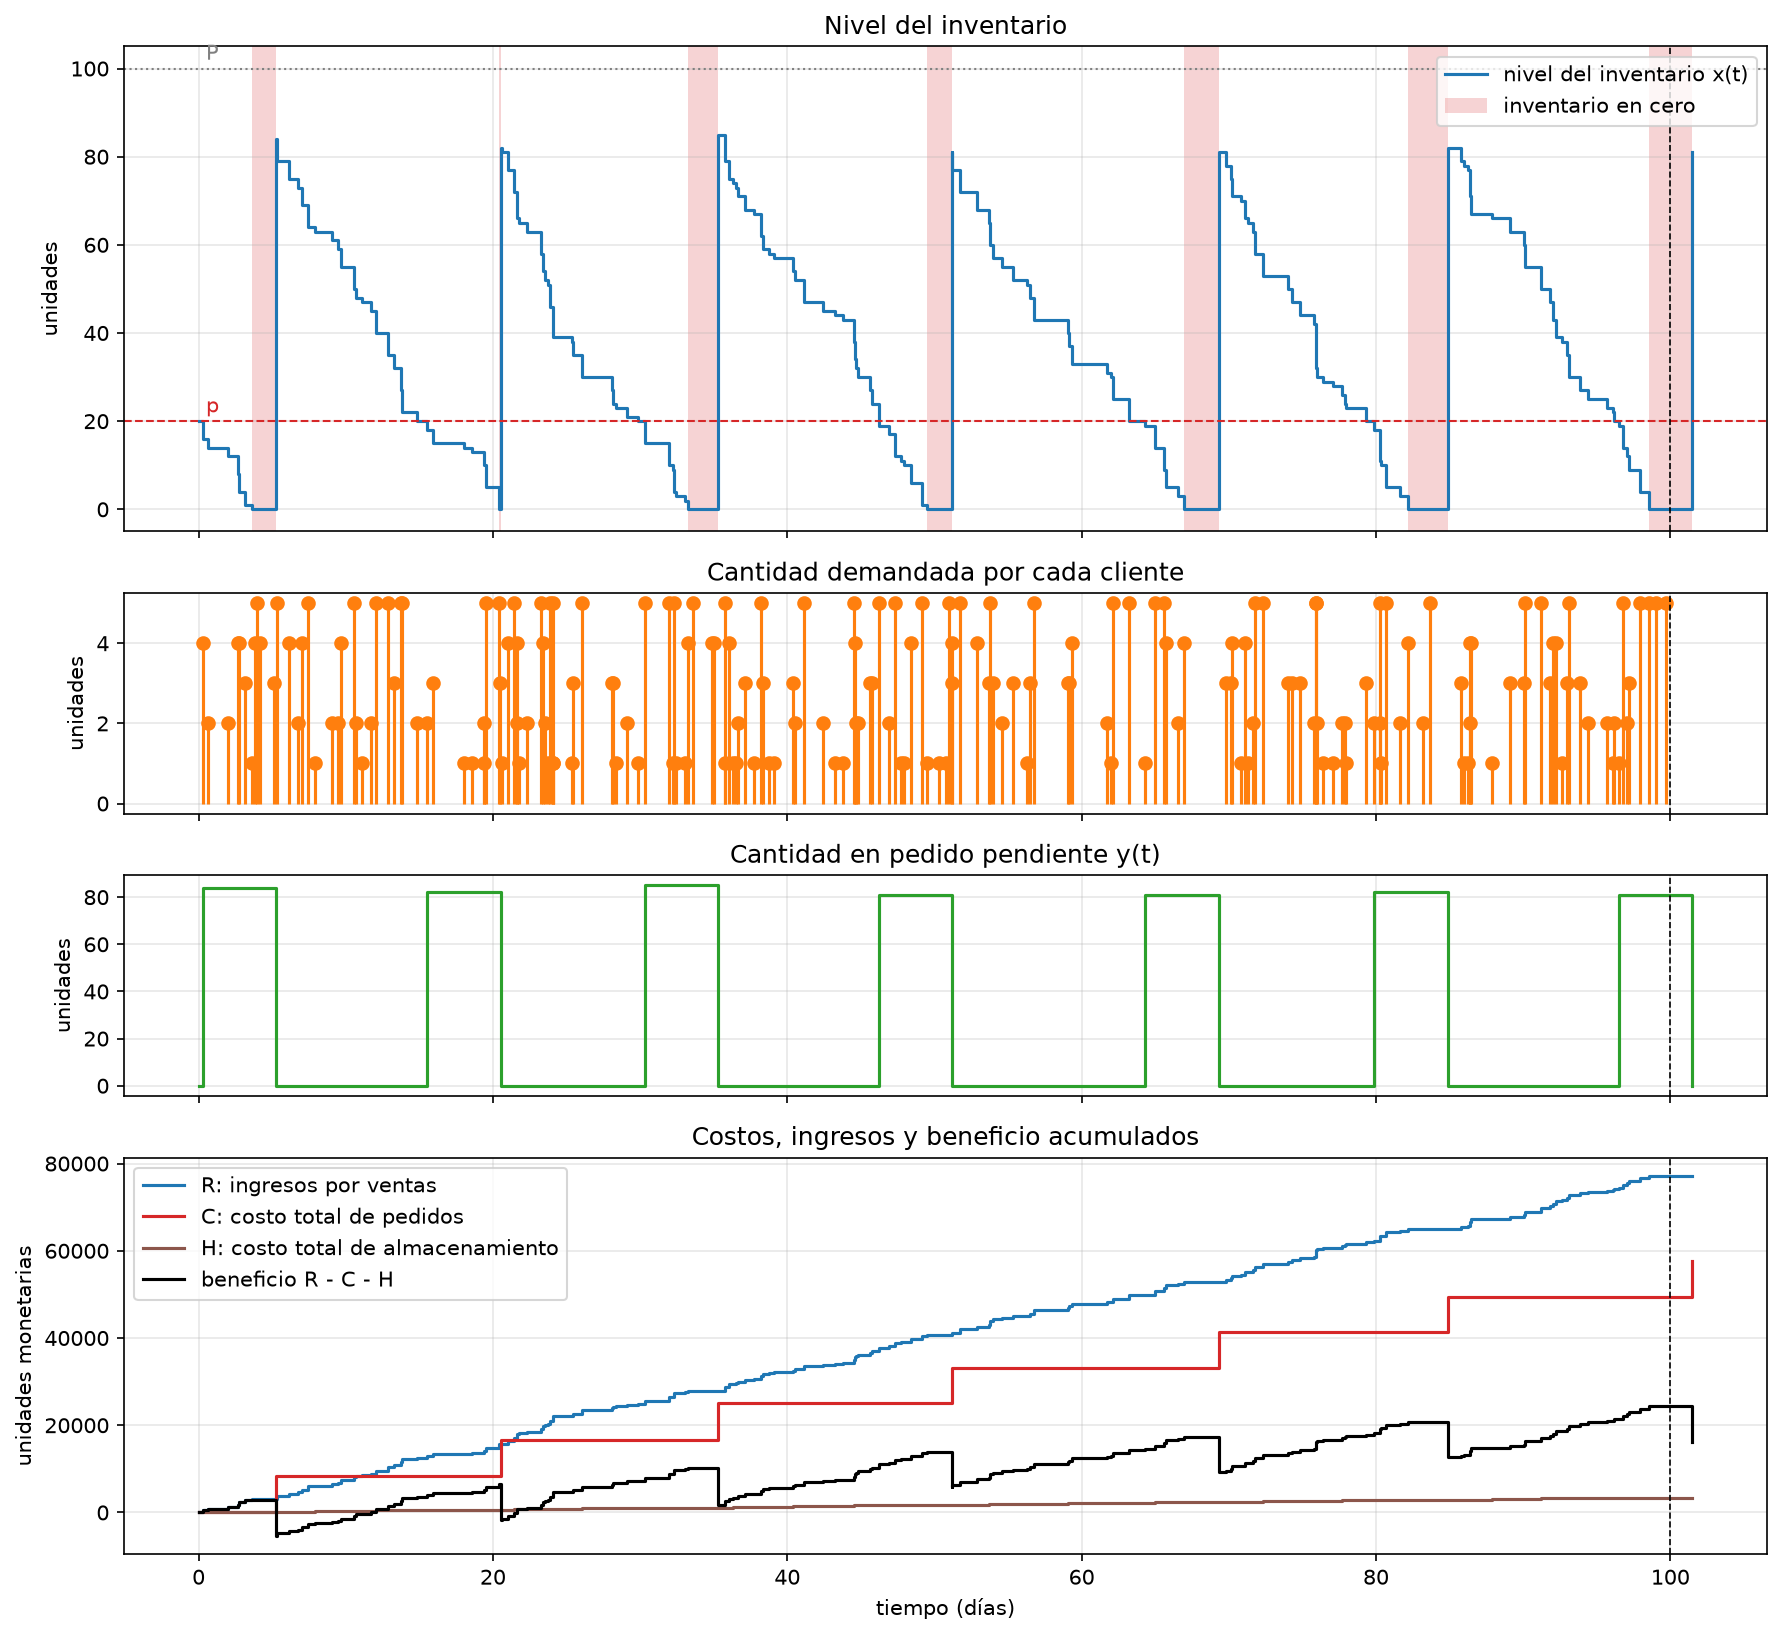
\includegraphics[width=\textwidth]{inventario_evolucion.png}
\caption{Evolución temporal del modelo de inventario (corrida base, $\lambda=2$): nivel del
inventario con los periodos en cero sombreados, demanda de cada cliente, pedido pendiente
y costos, ingresos y beneficio acumulados. La línea discontinua marca $T=100$.}\label{fig:inv}
\end{figure}

\begin{table}[H]\centering\small
\caption{Inventario: medidas de desempeño en 20 réplicas ($\lambda=2$, $p=20$).}\label{tab:inv}
\begin{tabular}{p{.45\textwidth}rrc}\toprule
\textbf{Medida}&\textbf{Media}&\textbf{Desv. est.}&\textbf{IC 95\,\%}\\\midrule
\inputtablerows{tablas/tabla_inventario.tex}
\bottomrule
\end{tabular}\end{table}

\begin{table}[H]\centering\small
\caption{Sensibilidad a $\lambda$: media $\pm$ semiancho del IC 95\,\% (20 réplicas).}\label{tab:inv_lambda}
\begin{tabular}{ccccc}\toprule
$\lambda$&\textbf{Demanda en $L$}&\textbf{Beneficio}&\textbf{\% satisfechos}&\textbf{\% en cero}\\\midrule
\inputtablerows{tablas/tabla_inventario_lambda.tex}
\bottomrule
\end{tabular}\end{table}

\begin{figure}[H]\centering
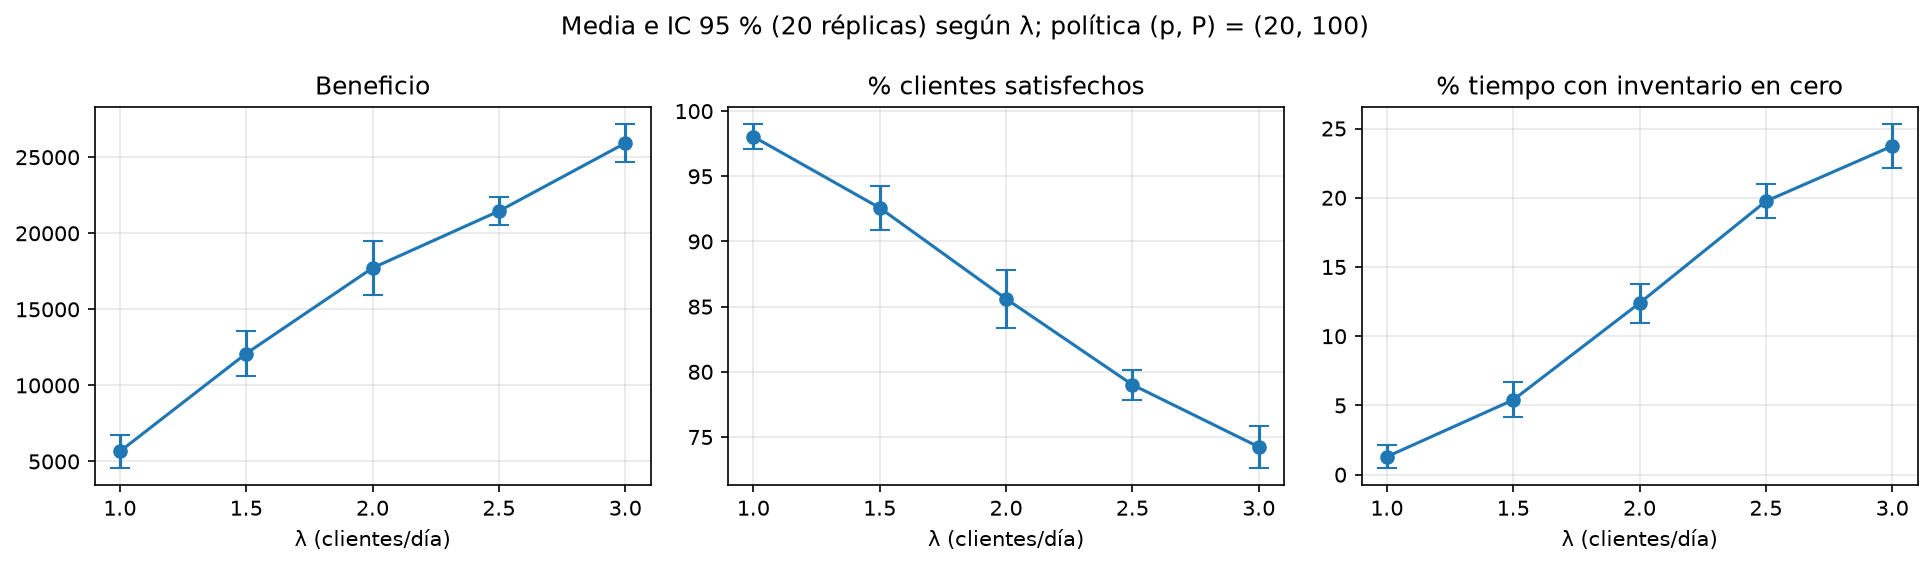
\includegraphics[width=\textwidth]{inventario_sensibilidad.png}
\caption{Medidas de desempeño según $\lambda$ con la política $(p,P)=(20,100)$.}\label{fig:inv_sens}
\end{figure}

\begin{table}[H]\centering\small
\caption{Efecto del punto de pedido $p$ con $\lambda=2$ (medias de 20 réplicas).}\label{tab:inv_p}
\begin{tabular}{cccccc}\toprule
$p$&\textbf{Beneficio}&\textbf{Benef.\ + $h\,x_{fin}$}&\textbf{$H$}&\textbf{\% satisf.}&\textbf{\% en cero}\\\midrule
\inputtablerows{tablas/tabla_inventario_p.tex}
\bottomrule
\end{tabular}\end{table}

\paragraph{Análisis.} El nivel del inventario sigue un diente de sierra. Cada pedido es de
unas 80--85 unidades, porque se lanza apenas $x$ baja de 20. El inventario nunca llega a
$P=100$, porque durante los cinco días de entrega sigue habiendo ventas. En casi todos los
ciclos hay una ruptura, ya que la demanda esperada durante la entrega (30) supera a $p$.
El costo de pedidos crece en escalones de unos 8\,000 y domina la estructura de costos; el
almacenamiento representa apenas el 4,5\,\% de los ingresos.

En las 20 réplicas (Tabla~\ref{tab:inv}), los porcentajes se estiman con precisión: se
satisface al 85,6\,\% de los clientes ($\pm2{,}2$ puntos) y el inventario está en cero el
12,4\,\% del tiempo ($\pm1{,}4$). El beneficio medio es 17\,718, con un semiancho relativo
del 9,9\,\%. Gran parte de esa variabilidad es un \emph{efecto de borde}: la política
sigue pidiendo cerca del final, y el último pedido se paga completo aunque sus unidades ya
no se venden dentro del horizonte. En la corrida base, el pedido que llega en $t=101{,}5$
reduce el beneficio de unos 24\,300 a 16\,217. La correlación entre beneficio e inventario
final es de $-0{,}80$. Si se valora el inventario final a su costo, el beneficio medio sube a
24\,258 y su desviación estándar baja de 3\,743 a 2\,283.

Al aumentar $\lambda$ (Tabla~\ref{tab:inv_lambda} y Figura~\ref{fig:inv_sens}), el beneficio
crece casi linealmente porque cada unidad vendida deja un margen positivo. Sin embargo, el
servicio cae de 98,0\,\% a 74,2\,\% y el tiempo sin inventario sube de 1,3\,\% a 23,7\,\%.
La política $(20,100)$ solo es adecuada cuando la demanda durante la entrega es menor que
$p$, como ocurre con $\lambda=1$. La Tabla~\ref{tab:inv_p} muestra que, con $\lambda=2$,
subir el punto de pedido a $p=40\approx\mu_L+\sigma_L$ eleva el servicio a 95,5\,\% y reduce
el tiempo en cero a 3,5\,\%. Además aumenta el beneficio, a cambio de un 12\,\% más de costo
de almacenamiento. Esta es la información que el empresario usaría para redefinir su
política de gestión del inventario, como plantea el libro.

\subsection{SimPy}
\begin{table}[H]\centering\small
\caption{Ejemplos oficiales de SimPy implementados.}\label{tab:simpy}
\begin{tabular}{p{.19\textwidth}p{.28\textwidth}p{.43\textwidth}}\toprule
\textbf{Ejemplo}&\textbf{Mecanismos}&\textbf{Resultado observado (semilla 42)}\\\midrule
Bank Renege&\texttt{Resource}, condición \texttt{req | timeout}&1 de 5 clientes abandona
la cola tras esperar 1,174.\\
Carwash&\texttt{Resource(2)}, espera de procesos&Los 4 carros iniciales se lavan en dos
tandas; ninguna espera supera 5 min.\\
Machine Shop&\texttt{PreemptiveResource}, \texttt{interrupt}&32\,775 piezas en 4 semanas
(81\,\% del máximo sin fallas).\\
Movie Renege&Evento compartido \texttt{sold\_out}&Las 3 películas se agotan entre los
minutos 28 y 43; 26 personas abandonan.\\
Gas Station&\texttt{Container}, proceso de control&El camión se llama a los 460 s y llega a
los 760 s; dos carros esperan combustible.\\
Process Comm.&\texttt{Store}, \texttt{BroadcastPipe}&Mensajes en buffer marcados como
tardíos; difusión a dos consumidores.\\
Event Latency&\texttt{Store}, proceso de retardo&Cada mensaje llega exactamente 10 unidades
después.\\\bottomrule
\end{tabular}\end{table}

Con la misma semilla, las salidas de Bank Renege y Machine Shop coinciden con las
publicadas en la documentación de SimPy, lo que confirma la fidelidad de la
implementación. Frente a las secciones anteriores, SimPy elimina la programación manual de
la lista de sucesos: basta con describir el ciclo de vida de cada entidad, y las colas, la
planificación y el reloj los gestiona el \texttt{Environment}. Sus primitivas cubren
directamente patrones que a mano serían costosos: abandono por impaciencia, prioridades con
expropiación, niveles continuos (\texttt{Container}), paso de mensajes y eventos que afectan
a muchos procesos a la vez.

\subsection{AnyLogic}
Las 40 corridas alcanzaron sus horizontes completos. En todas se verificó que las
entradas admitidas son iguales a las salidas más el trabajo pendiente, y que las
salidas son iguales a las unidades conformes más las rechazadas.

\begin{table}[H]\centering\small
\caption{Resultados de AnyLogic: media e intervalo de confianza del 95\,\%.}
\begin{tabular}{lrr}\toprule
Medida & Job Shop (8 h) & Baterías (4 h)\\\midrule
Producción conforme (unidades/h) & 55,66 [55,40; 55,91] & 8,35 [7,80; 8,90]\\
Ciclo de salidas (min) & 57,12 [56,07; 58,18] & 21,12 [17,30; 24,94]\\
WIP medio (unidades) & 57,31 [56,32; 58,31] & 3,28 [2,47; 4,09]\\
WIP final (unidades) & 34,75 [32,71; 36,79] & 3,60 [2,23; 4,97]\\
Utilización del recurso (\%) & 95,83 [95,75; 95,91] & 92,84 [91,46; 94,22]\\\bottomrule
\end{tabular}\end{table}

Job Shop terminó en promedio 445,25 de los 480 pallets admitidos. Baterías entregó
33,4 unidades conformes por corrida. En las 20 réplicas de baterías se observaron
tres rechazos entre 671 salidas: 0,447\,\%, con IC de Wilson del 95\,\% de
[0,152; 1,306]\,\%. El número de rechazos es pequeño para validar con precisión
el 1\,\% configurado. Este IC binomial agrupado difiere del IC t entre réplicas.

El ciclo se mide desde la admisión en Source hasta Sink y solo incluye las salidas
anteriores al horizonte. En baterías comienza con la admisión de la caja; no representa
el tiempo total desde la fabricación del electrodo. El WIP medio se calcula por
integración temporal. La utilización corresponde a los CNC y al operador de ensamblaje,
respectivamente, e incluye períodos de reserva del recurso. En Job Shop se reserva el
CNC antes de recuperar el pallet: su utilización no equivale al porcentaje de tiempo
de mecanizado. Son resultados transitorios desde vacío, sin calentamiento; los
horizontes distintos impiden una comparación directa entre los procesos.

\begin{figure}[H]\centering
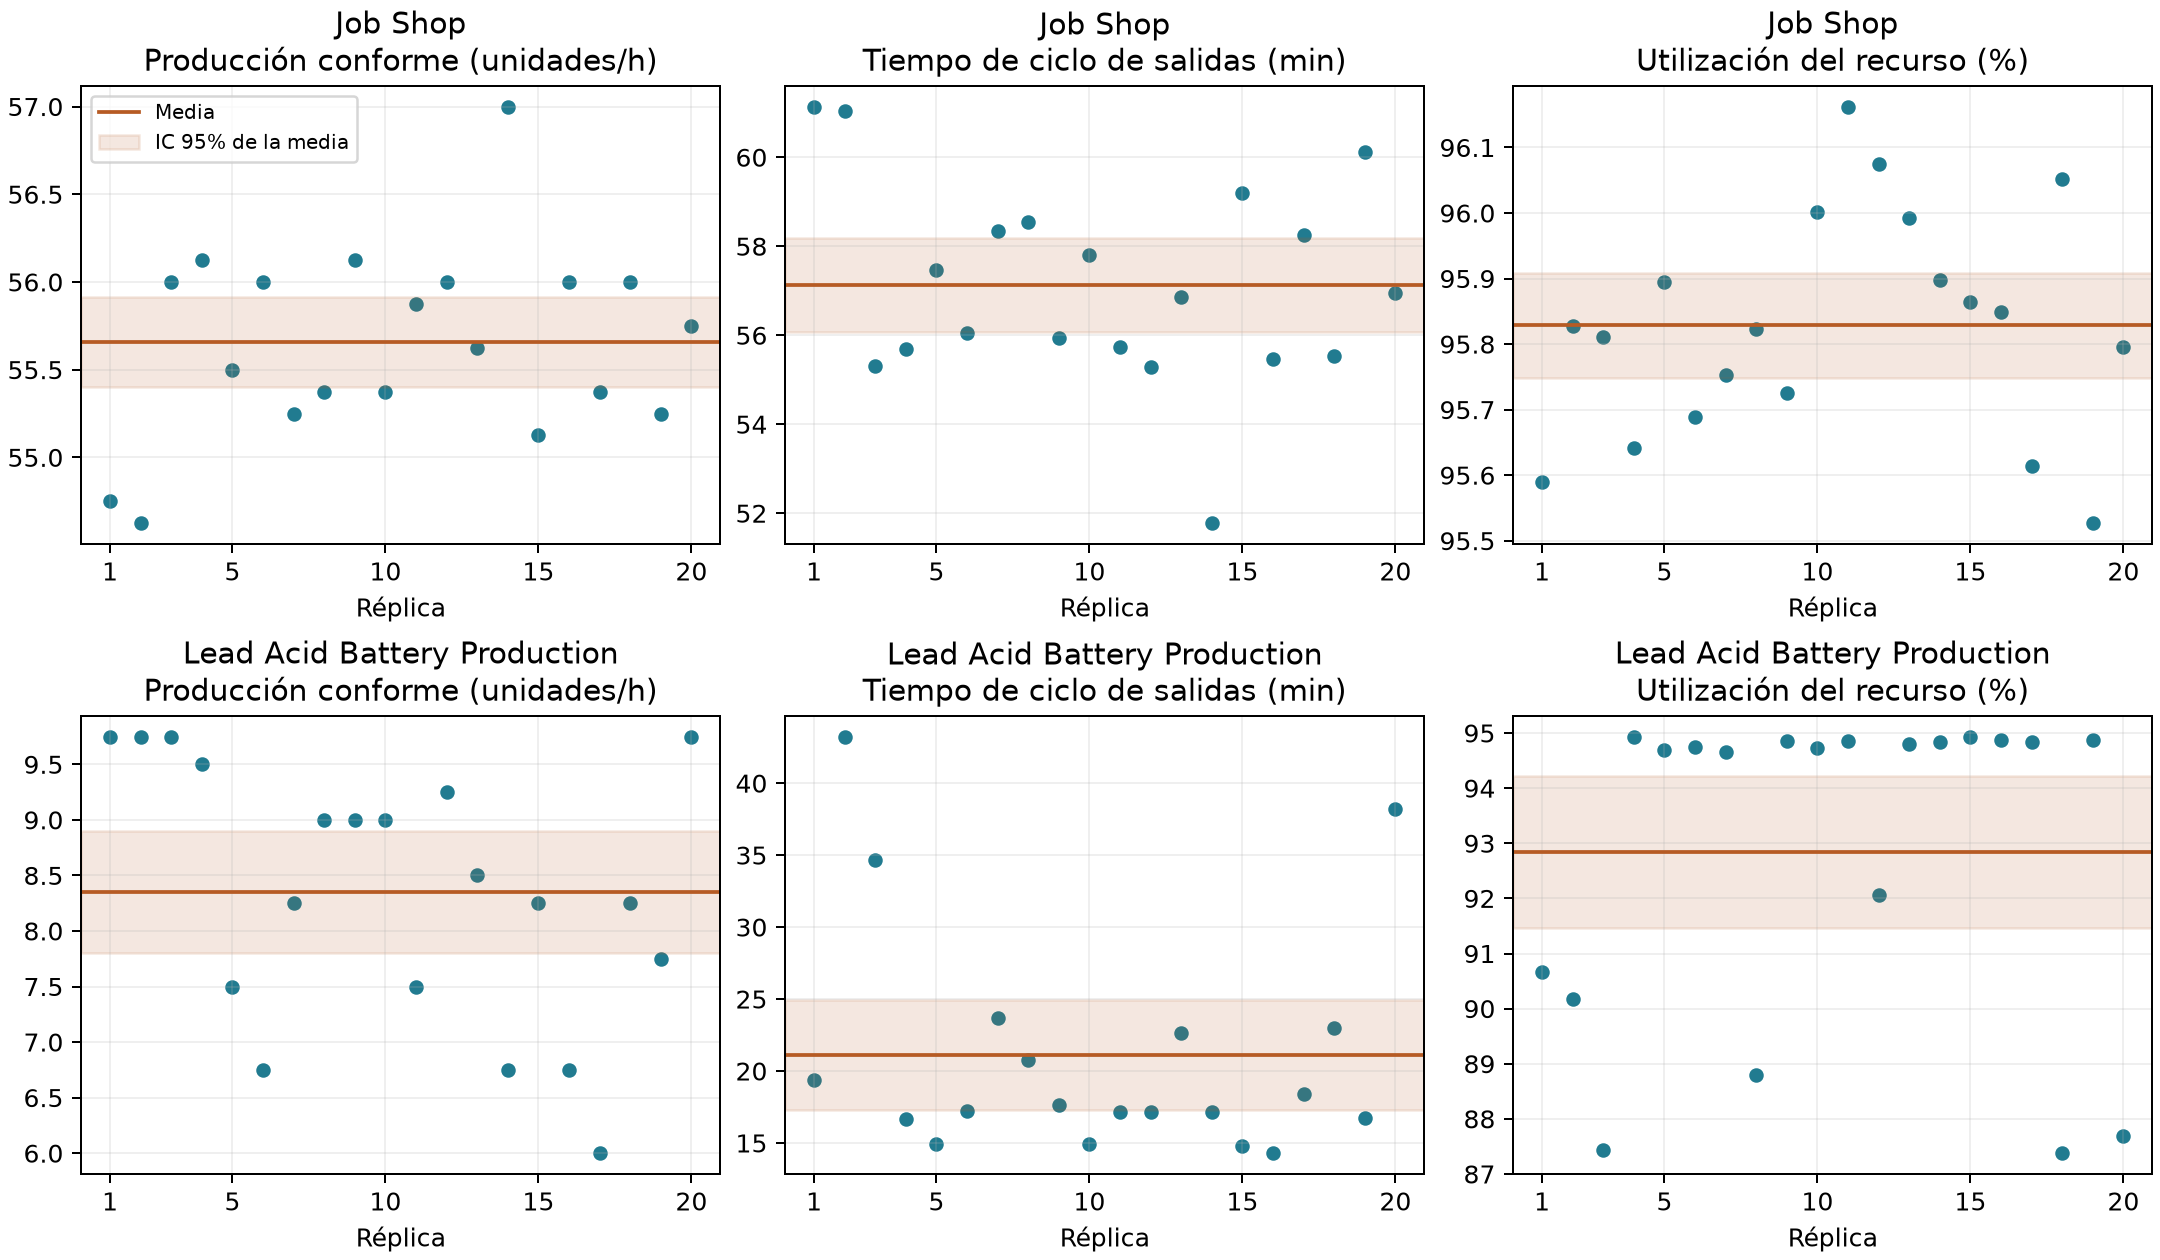
\includegraphics[width=\textwidth]{anylogic/estadistica_ic95.png}
\caption{Réplicas de AnyLogic. La línea indica la media y la banda el IC del 95\,\%
de la media, no el intervalo de variación de una corrida individual.}
\end{figure}

Los modelos, fases, instrucciones y metodología completa están en
\texttt{anylogic\_models}; los datos originales y resúmenes están en
\texttt{datos/anylogic}. Las capturas de las 20 réplicas completadas se guardaron en
\texttt{imagenes/anylogic}.

\section{Conclusiones}
\begin{itemize}
 \item La programación de sucesos (estado, lista de sucesos y rutinas) permitió reproducir
 y corregir los modelos G/G/1 y de red de colas. Se identificaron errores de índices y de
 acumulación de áreas en los notebooks base que sesgaban los tiempos medios y el número
 medio de clientes.
 \item Todos los escenarios de la G/G/1 y el escenario A de la red tienen intensidad de
 tráfico mayor que uno. En ellos, las medidas dependen del horizonte y una aproximación de
 flujo predice bien la cola acumulada, el tiempo de vaciado y la espera media.
 \item La utilización de cada nodo identifica el cuello de botella: el nodo 3 en el
 escenario A. En el escenario B, el servicio dependiente del estado estabiliza el nodo 3.
 \item En el inventario, la política $(p,P)=(20,100)$ es insuficiente para $\lambda\ge1{,}5$,
 porque el punto de pedido es menor que la demanda esperada durante la entrega. Fijar $p$
 cerca de $\mu_L+\sigma_L$ mejora a la vez el servicio y el beneficio. El beneficio de
 horizonte finito está sesgado por los pedidos que llegan al final, así que conviene valorar
 el inventario remanente.
 \item Las réplicas independientes y los intervalos $t$ cuantifican la incertidumbre. Los
 conteos se estiman con precisión, mientras que las medidas de congestión de nodos críticos
 requieren muchas más réplicas.
 \item SimPy simplifica la construcción de modelos de eventos discretos mediante procesos
 y recursos, y los siete ejemplos reprodujeron las salidas de referencia.
\end{itemize}

\begin{thebibliography}{9}
\bibitem{rios2008} D. Ríos Insua, S. Ríos Insua y J. Martín, \textit{Simulación: métodos
y aplicaciones}, 2.ª ed. Alfaomega, 2008, cap. 5.
\bibitem{simpydocs} Team SimPy, \textit{SimPy: Discrete event simulation for Python},
documentación v4.1. \url{https://simpy.readthedocs.io}
\bibitem{scherfke2014} S. Scherfke, \textit{Discrete-event simulation with SimPy},
EuroPython 2014. \url{https://stefan.sofa-rockers.org/downloads/simpy-ep14.pdf}
\bibitem{anylogichelp} The AnyLogic Company, \textit{AnyLogic Help: Tutorials}.
\url{https://anylogic.help/tutorials/}
\end{thebibliography}
\end{document}
